\documentclass{beamer}
\usetheme{default}
\usepackage{tikz}
\usepackage{graphicx}
\usepackage{pgfplots}
\usepackage{subcaption}
\usepackage{siunitx}
\usepackage{caption}
\usepackage{chemformula}
\usepackage[ngerman]{babel}
\pgfplotsset{width=\textwidth, every axis/.append style={
                    axis x line=middle,    % put the x axis in the middle
                    axis y line=middle,    % put the y axis in the middle
                    axis line style={->}, % arrows on the axis
                    xlabel={$x$},          % default put x on x-axis
                    ylabel={$y$},          % default put y on y-axis
                    font=\tiny
            }}

%\captionsetup[format=hang]

\AtBeginSection[]{
  \begin{frame}
  \vfill
  \centering
  \begin{beamercolorbox}[sep=8pt,center,shadow=true,rounded=true]{title}
    \usebeamerfont{title}\insertsectionhead\par%
  \end{beamercolorbox}
  \vfill
  \end{frame}
}

\title{Quanten-Hall-Effekt}
\author{Michael Rößner \and Jonas Schambeck}

\begin{document}
    \maketitle
    \frame{\frametitle{Inhalt}\tableofcontents}

\section{2D Elektronengas}
\begin{frame}
    \frametitle{Definition}

\begin{itemize}
    \item Elektronen in konstantem Potential delokalisiert
    \item In Potenzialbarriere (Probenrand) eingesperrt
    \item Pauliprinzip für Elektronen: Ein Teilchen pro Zustand
\end{itemize}

\begin{figure}
    \begin{subfigure}[c]{0.4\textwidth}
        \begin{tikzpicture}
            % Potential
            \draw (1,1) node {\tiny Probe};
            \draw [thick] [<-](0.1,1) -- (0.6,1);
            \draw [thick] [->] (1.4,1) -- (1.9,1);
            \draw [thick]%
            (-0.2,2) -- (0,2) -- (0,0) -- (2,0) -- (2,2) -- (2.2,2);
            \draw (1,0) node[anchor=north] {\tiny x};
            \draw (0,1.7) node[anchor=east] {\tiny U};
        \end{tikzpicture}
        \caption{Potentialverlauf der Probe}
    \end{subfigure}
    \begin{subfigure}[c]{0.4\textwidth}
        \begin{tikzpicture}
            \begin{axis}[%
                    xlabel={$E-E_F$},
                    ylabel={$f(E)$},
                    domain=-1:1,
                    ymin=-0.2,
                    ymax=1.2,
                    axis y line=left,
                    grid=both
            ]
                \addplot[color=blue]%
                {1/(exp(x/0.00086)+1)};
            \end{axis}
        \end{tikzpicture}
        \caption{Zustandsverteilung im Elektronengas}
    \end{subfigure}
\end{figure}
\end{frame}

\begin{frame}
    \frametitle{Herstellung}

\begin{itemize}
    \item Halbleiter-Heterostruktur aus Materialien mit unterschiedlichen Bandlücken
    \begin{itemize}
        \item Im Versuch: \ch{GaAs} ($\SI{1.4}{\eV}$) \& \ch{AlGaAs} ($1.4- \SI{2.2}{\eV}$)
    \end{itemize}
    \item Angleichen der Fermi-Niveaus bei Kontakt 
    \item Wanderung der Elektronen aus n-dot. \ch{AlGaAs:Si} in reines \ch{GaAs} in tief liegenden Potentialtopf
    \item Sehr hohe Beweglichkeit durch hohe Ladungsträgerdichte in weitgehend defektfreiem Material
\end{itemize}

\begin{figure}
    \begin{subfigure}[c]{0.4\textwidth}
    \begin{tikzpicture}[scale=1.1]
        % Heterostruktur Aufbau
        \draw (0,0) rectangle (1,1.8);
        % Striche
        \draw (0,0.6) -- (1,0.6);
        \draw (0,1.2) -- (1,1.2);
        \draw (0,1.5) -- (1,1.5);
        % 3D Striche
        \draw (0,1.8) -- (0.1,1.9);
        \draw (1,1.8) -- (1.1,1.9);
        \draw (1,1.5) -- (1.1,1.6);
        \draw (1,1.2) -- (1.1,1.3);
        \draw (1,0.6) -- (1.1,0.7);
        \draw (1,0) -- (1.1,0.1);
        % Beschriftung
        \draw (0.5,0.25) node {\tiny \ch{GaAs}};
        \draw (0.5,0.9) node {\tiny \ch{AlGaAs}};
        \draw (0.5,1.35) node {\tiny \ch{AlGaAs:Si}};
        \draw (0.5,1.65) node {\tiny \ch{GaAs}};
        % gestrichelte Linien
        \draw [dashed] (1,1.65) -- (1.5,1.65);
        \draw [dashed] (1,1.35) -- (1.5,1.35);
        \draw [dashed] (1,0.9) -- (1.5,0.9);
        % Beschriftung aussen
        \draw (1.5,1.65) node[anchor=west] {\tiny Deckschicht};
        \draw (1.5,1.35) node[anchor=west] {\tiny Dotierschicht};
        \draw (1.5,0.9) node[anchor=west] {\tiny Spacer};
    \end{tikzpicture}
    \end{subfigure}
    \begin{subfigure}[c]{0.4\textwidth}
        \begin{tikzpicture}[scale=1.05]
            % Halbleiter A
            \draw (1.5, 0) rectangle (2.5,1);
            \draw (1.5, 0.2) -- (2.5,0.2);
            \draw (1.5,0.8) -- (2.5,0.8);
            \draw [dashed] (1.5,0.65) -- (2.5,0.65);
            \draw (1.5,0.65) node[anchor=east] {\tiny $E_F$};
            \draw (2,0.9) node {\tiny A};
            % Halbleiter B
            \draw (2.5, 0) rectangle (3.5,1);
            \draw (2.5, 0.35) -- (3.5,0.35);
            \draw (2.5,0.65) -- (3.5,0.65);
            \draw [dashed] (2.5,0.5) -- (3.5,0.5);
            \draw (3.5,0.5) node[anchor=west] {\tiny $E_F$};
            \draw (3,0.9) node {\tiny B};
            % Heterostruktur
            \draw (1.5,-1.3) rectangle (3.5,-0.3);
            \draw [dashed] (1.5,-0.7) -- (3.5,-0.7);
                % Leitungsband
            \draw (1.5,-0.5) -- (2.3,-0.5);
            \draw (2.3,-0.5) to[bend right] (2.5,-0.4); 
            \draw (2.5,-0.4) -- (2.5,-0.8);
            \draw (2.5,-0.8) to[bend left] (2.8,-0.65);
            \draw (2.8,-0.65) -- (3.5,-0.65);
            \draw (2.5,-0.7) -- (2.6,-0.7);
                % Valenzband
            \draw (1.5,-1.1) -- (2.45,-1.1);
            \draw (2.45,-1.1) to[bend right] (2.5, -1.0);
            \draw (2.5,-1.0) to[bend left] (2.6,-0.9);
            \draw (2.6,-0.9) -- (3.5,-0.9);
                % Beschriftung
            \draw (2.3,-0.8) -- (2.53,-0.73);
            \draw (2.4,-0.85) node[anchor=east] {\tiny 2DEG};
            \draw (1.5,-0.7) node[anchor=east] {\tiny $E_F$};
        \end{tikzpicture}
    \end{subfigure}
\end{figure}

\end{frame}

\begin{frame}
    \frametitle{Zustandsdichte (DOS)}
    \begin{itemize}
        \item Beschreibt Anzahl besetzter Zustände pro Energie und Volumen
        \item DOS für 2D Systeme: 
              $D^{(2)} (E) = \frac{m}{\pi \hbar^2}$ konstant!
        \item Aufspaltung der Dispersionskurve in Subbänder auf\\
              $\Rightarrow$ Stufen konstanter DOS mit Abstand $\frac{m}{\pi\hbar^2}$
    \end{itemize}

\begin{figure}
    \begin{subfigure}[c]{0.6\textwidth}
    \begin{tikzpicture}
        \begin{axis}[%
                ymax=3,xmin=0.5,
                ticks=none,
                xlabel={E}, ylabel={D(E)}
        ]
            \addplot[thick,blue] coordinates {(1,0)(1,0.5)(1.5,0.5)(1.5,1)(2.25,1)(2.25,1.5)(3.25,1.5)(3.25,2)(4.75,2)};
        \end{axis}
    \end{tikzpicture}
    \end{subfigure}
\end{figure}
\end{frame}

\section{Hall-Effekt}
\begin{frame}
    \frametitle{Hallprobe}
\begin{itemize}
    \item Stromfluss in x-Richtung durch Probe (P)
    \item B-Feld in z-Richtung
    \item Messung der Längsspannung $U_{xx}~(2\rightarrow3)$ und Hall-Spannung
          $U_H~(3\rightarrow5)$
    \item Aus Widerstandstensoren: $R_H = \frac{U_H}{I}$, 
          $R_\square = \frac{U_{xx}}{I} \frac{W}{L}$
\end{itemize}
\begin{figure}
    \begin{subfigure}[c]{0.4\textwidth}
    \begin{tikzpicture}
        % Koordinaten
        \draw [<->] (-0.2,-0.7) -- (-0.2,-1.2) -- (0.3,-1.2);
        \draw (-0.15,-1.15) -- (-0.25,-1.25);
        \draw (-0.15,-1.25) -- (-0.25,-1.15);
        \draw (0.3,-1.23) node[anchor=south] {\tiny x};
        \draw (-0.2,-0.75) node[anchor=west] {\tiny y};
        \draw (-0.25,-1.17) node[anchor=north] {\tiny z};
        % Rahmen
        \draw [very thick] (-0.5,-1.5) rectangle (3.5,1.5);
        %Bauelemente
        \draw (0,0) node[rectangle,draw] {1};
        \draw (2,0) node[rectangle,draw] {P};
        \draw (3,0) node[rectangle,draw] {4};
        \draw (1.75, 1) node[rectangle,draw] {2};
        \draw (2.25, 1) node[rectangle,draw] {3};
        \draw (1.75,-1) node[rectangle,draw] {6};
        \draw (2.25,-1) node[rectangle,draw] {5};
        % W, L
        \draw (1.6, 0  ) node {\tiny W};
        \draw (2  ,-0.4) node {\tiny L};
        % Kabel 1
        \draw (0.22,-0.2) -- (1.75,-0.2);
        \draw (0.22,0.2) -- (1.75,0.2);
        % Kabel 4
        \draw (2.25,-0.2) -- (2.78,-0.2);
        \draw (2.25, 0.2) -- (2.78, 0.2);
        % Kabel 2
        \draw (1.75,0.75) -- (1.75,0.5);
        \draw (1.75, 0.5) -- (1.9,0.5);
        \draw (1.9 , 0.5) -- (1.9,0.25);
        % Kabel 3
        \draw (2.25,0.75) -- (2.25,0.5);
        \draw (2.25, 0.5) -- (2.1,0.5);
        \draw (2.1 , 0.5) -- (2.1,0.25);
        % Kabel 6
        \draw (1.75,-0.75) -- (1.75,-0.5);
        \draw (1.75,- 0.5) -- (1.9, -0.5);
        \draw (1.9 ,- 0.5) -- (1.9, -0.25);
        % Kabel 3
        \draw (2.25,-0.75) -- (2.25,-0.5);
        \draw (2.25,- 0.5) -- (2.1, -0.5);
        \draw (2.1 ,- 0.5) -- (2.1, -0.25);
    \end{tikzpicture}
    \end{subfigure}
\end{figure}
\end{frame}

\begin{frame}
    \frametitle{Definition}
\begin{itemize}
    \item Aus klassischer statischer BGL mit $\vec{B} = (0,0,B)$ errechnet man:
          \[R_H = \frac{B}{n_s \, e} \qquad R_\square = \frac{1}{n_s \, e \, \mu}\]
          $n_s$: Ladungsträgerdichte, $e$: Elementarladung, $\mu$: Beweglichkeit
\end{itemize}
\begin{figure}
    \begin{subfigure}[c]{0.45\textwidth}
        \begin{tikzpicture}
            \begin{axis}[
                ticks=none,
                xlabel={$T$}, ylabel={$R_H$},
                grid=both
            ]
                \addplot[thick, blue] {x};
            \end{axis}
        \end{tikzpicture}
        \caption{Hall-Widerstand}
    \end{subfigure}
    \begin{subfigure}[c]{0.45\textwidth}
        \begin{tikzpicture}
            \begin{axis}[
                ticks=none,
                xlabel={$T$}, ylabel={$R_\square$},
                grid=both
            ]
                \addplot[thick, blue] {1};
            \end{axis}
        \end{tikzpicture}
        \caption{Schichtwiderstand}
    \end{subfigure}
\end{figure}
\end{frame}

\begin{frame}
    \frametitle{Quanten-Hall-Effekt}
\begin{itemize}
    \item Auftreten von Quanteneffekten bei sehr tiefen Temperaturen und starken
          Magnetfeldern
\end{itemize}
\begin{figure}
    \begin{subfigure}[c]{0.6\textwidth}
        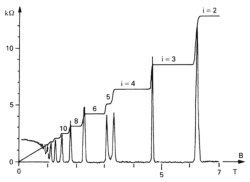
\includegraphics[width=\textwidth]{quantum-hall-effect.pdf}
        \caption{Widerstände mit Quanteneffekten}
    \end{subfigure}
\end{figure}
\end{frame}

\begin{frame}
    \frametitle{Landau-Level}
\begin{itemize}
    \item Quantelung der Elektronenenergie im homogenen Magnetfeld
          \[E_n = \left(n+\frac{1}{2} \right) \hbar \omega_c, 
          \quad \omega_c = \frac{eB}{m^*}\]
    \item Energiewerte der \glqq Landauniveaus/-levels\grqq
\end{itemize}

\begin{figure}
    % Parabel
    \begin{subfigure}[c]{0.33\textwidth}
    \begin{tikzpicture}
        % Koordinatensystem
        \draw [->] (0,-0.25) -- (0,2);
        \draw [->] (-1,0) -- (1.25,0);
        \draw (0,2) node[anchor=west] {\tiny $E$};
        \draw (1.25,0) node[anchor=north] {\tiny $k_x$};
        % Funktion
        \draw[domain=-0.9:0.9] plot ({\x}, {2*\x*\x+0.2});
        % Beschriftung
        \draw [dashed] (-0.37,0.52) -- (0.4,0.52);
        \draw [dashed] (-0.6, 0.92) -- (0.6,0.92);
        \draw [dashed] (-0.748,1.32) --(0.748,1.32);
        \draw [<->] (0.7,0.52) -- (0.7,0.92);
        \draw (0.7,0.72) node[anchor=west] {\tiny $\hbar \omega_c$};
    \end{tikzpicture}
    \caption{Diskrete Zustände bei Energiewerte, der Landauniveaus}
    \end{subfigure}
    % Kreise
    \begin{subfigure}[c]{0.33\textwidth}
    \begin{tikzpicture}
        % Koordinatensystem
        \draw [->] (-1.25,0) -- (1.4,0);
        \draw [->] (0,-1.25) -- (0,1.4);
        \draw (1.4,0) node[anchor=north] {\tiny $k_x$};
        \draw (0,1.4) node[anchor=west] {\tiny $k_y$};
        % Kreise
        \draw (0,0) circle (10pt);
        \draw (0,0) circle (20pt);
        \draw (0,0) circle (30pt);
        % Zustände
        \foreach \r in {0.35,0.7,1.05}{
            \foreach \x/\y in {0/1,1/0,-1/0,
                               0.8660254037844387/0.49999999999999994,% pi/6
                               0.49999999999999994/0.8660254037844387,% pi/3
                               -0.4999999999999998/0.8660254037844387,
                               -0.8660254037844387/0.49999999999999994
            }{
                \pgfmathsetmacro{\test}{1-(\x*\x)}
                \draw [fill] (\r*\x,\r*\y) circle (1pt);
                \draw [fill] (\r*\x,-\r*\y) circle (1pt);
            }
        }
    \end{tikzpicture}
    \caption{Zustände kondensieren auf Kreislinien}
    \end{subfigure}
    % Energiediagramm
    \begin{subfigure}[c]{0.3\textwidth}
        \begin{tikzpicture}[scale=1.2]
            \begin{axis}[xmin=0,xmax=4.5,ymax=1.2,
                xlabel={$E$},ylabel={$D(E)$},
                x label style={at={(current axis.right of origin)},
                               anchor=north,below=-0mm,left=-0.5mm},
                y label style={at={(current axis.above origin)},
                               anchor=south,below=-2mm},
                ticks=none]
                \addplot[blue] coordinates {(1,0)(1.1,1)(1.2,0)} ;
                \addplot[blue] coordinates {(2,0)(2.1,1)(2.2,0)} ;
                \addplot[blue] coordinates {(3,0)(3.1,1)(3.2,0)} ;
            \end{axis}
            \draw [<->] (0.8,0.95) -- (1.1,0.95);
            \draw (0.95,0.95) node[anchor=south] {\tiny $\hbar \omega_c$};
        \end{tikzpicture}
    \caption{Zustandsdichte spaltet in diskrete Landauniveaus auf}
    \end{subfigure}
\end{figure}

\end{frame}

\end{document}
